\documentclass[a4paper,10pt]{article}
\usepackage[utf8]{inputenc}
\usepackage{graphicx}
\usepackage[english]{babel}
\usepackage[margin=0.5in]{geometry}

\title{EECS 568 Final Project Proposal}
\author{Ali Abdallah, Alex Crean, Mohamad Wajih Farhat, Alexander Groh,  \\  Steven Liu, Chris Wernette}
\date{March 12, 2018}

\begin{document}

\maketitle

\section{Introduction}
We are motivated by the V-LOAM algorithm \cite{zhang2015visual} which is a trajectory oriented SLAM algorithm. We will apply this algorithm to autonomous vehicle (AV) applications. The V-LOAM algorithm uses high frequency camera based odometry for the motion prior that is corrected with high precision, low frequency lidar odometry as shown in Figure 1. We will use the KITTI dataset to benchmark our algorithm. The KITTI dataset includes ground truth measurements so we will measure our trajectory against it to measure our success.

\begin{figure}[h]
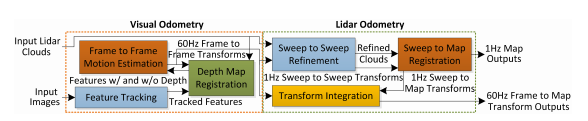
\includegraphics[width=12cm]{Algo}
\centering
\caption{VLOAM Algorithm, \cite{zhang2015visual}}
\end{figure}

We will implement Visual Odometry and lidar Correction to determine the trajectory. We plan on projecting our AV into a 3D point cloud of the lidar data for visualization of the pose. We plan on implementing this in MATLAB and possibly extend this to C++ for real time implementation because the MATLAB environment is substantially slower. 


\section{Milestone Goals}
Our first goal is to implement visual odometry SLAM on KITTI dataset. This involves frame to frame motion estimation, feature tracking, and depth map registration. We would like to validate this using the ground truth data from the KITTI dataset to try to minimize error. Second, we would like to concurrently work on the lidar algorithms which involves sweep to sweep refinement, transform integration, and sweep to map registration given the ground truth data as input. This way we can split up tasks to implement the two main parts of the algorithm in parallel and use the ground truth data as a sanity check of our algorithm. 
 
\section{Viability}
This algorithm has been implemented and proven with the KITTI dataset as the best algorithm used with that dataset. However, one of the issues with trajectory oriented SLAM is that we have to store the entire trajectory in our state. This causes our state to grow unboundedly, but it is something we will investigate and address throughout the project. In addition, this type of SLAM does not use loop closure to address drift, but it has the lowest drift among the algorithms benchmarked using KITTI. We will explore how much drift accumulates over long distances traveled.

\section{Foreseeable Difficulties}
The disadvantages of this algorithm are it requires creating an infinitely growing trajectory vector. We also assume that this algorithm is computationally intense, so it will have a slower update rate than other algorithms. A downside is that in dynamic environments you may have to update your vehicle faster than the algorithm is capable in order to have a safe algorithm.

\medskip

\bibliographystyle{unsrt}%Used BibTeX style is unsrt
\bibliography{references}

\end{document}